\documentclass{article}

\usepackage[hidelinks]{hyperref}

\usepackage{tikz}
\usetikzlibrary{matrix,chains,positioning,decorations.pathreplacing,arrows}

\usepackage{minted}
\usemintedstyle{colorful}

\addtolength{\oddsidemargin}{-.875in}
\addtolength{\evensidemargin}{-.875in}
\addtolength{\textwidth}{1.75in}

\addtolength{\topmargin}{-.875in}
\addtolength{\textheight}{1.75in}

\bibliographystyle{plain}

\begin{document}

\title{An Exploration of Neural Networks as Applied to Written Language Classification}
\author{Erik Boesen, Candidate gsg256}
\maketitle

\begin{abstract}
We assess the extent to which artificial neural networks can be used to perform recognition of written languages (conveyed through standard Unicode text rather than as graphically recognized handwriting or type). We use an artificial deep neural network to achieve a success rate of [Insert] at distinguishing between 8 different languages following supervised training.
\end{abstract}

\section{Introduction}
In this research we seek to develop and implement a neural network which differentiates between the world's 8 most common first languages according to \cite{ethnologue}, namely: Chinese, Spanish, English, Arabic, Hindi, Bengali, Portuguese, and Russian (ISO 639-1 alpha-2 codes zh, es, en, ar, hi, bn, pt, ru) \cite{iso639}. We explain the basics of neural networking techniques implemented, and give implementation examples using C++ (explaining and keeping to a minimum any idiomatic syntax).

\subsection{Training Data}
To train our network, we use dumps of article contents in the selected languages from the Wikimedia Foundation, obtained from \cite{wikidumps} as recommended in \cite{langsamp}. % Remove second citation?

For each language, data was retrieved from the 2018-04-20 dump, using the format ``Articles, templates, media/file descriptions, and primary meta-pages.'' These dump files are retrievable at \url{https://dumps.wikimedia.org/enwiki/20180420/enwiki-20180420-pages-articles.xml.bz2} (English, with the same URI format used for other languages). Chinese, Spanish, English, Portuguese, and Russian have Wikimedia databases too large to be practically handled; thus, we use only a single chunk of those databases, which are hosted at inconsistent URIs. We use a simple bash script to download and extract data in each language, then a Python program to extract article text from the raw XML files and parse it to remove markup characters \cite{parsewikixml}. Both programs may be found in \hyperref[sec:appendix_a]{Appendix A}.

\subsection{A general overview of neural networks}
\subsubsection{Why use a Neural Network?}
Neural Networks are a common technique used in the burgeoning field of machine learning. Machine learning techniques are useful when a large and diverse set of data must be processed (often entailing categorization), but when writing explicit code to make distinctions between data points would be impractical. For example, when identifying objects in an image, as in \cite{hinton12}, it would be nearly impossible to write a procedure to directly read image data and distinguish between many images. Though there exist simpler machine learning techniques, such as the K Nearest Neighbors algorithm, these strategies have trouble making decisions in so many dimensions with such a complex output vector as demonstrated in \cite{knnic}. Though the concept of a neural network was first proposed in 1958 \cite{rosenblatt58}, the concept has recently experienced a resurgence of popularity. Machine learning techniques based on neural networks including deep learning [citation needed] and recurrent neural networks [citation needed] have recently been applied to diverse problems, including achieving victory over a human in the age-old game of Go [citation needed], differentiating between multiple thouands of different image classes \cite{hinton12}, and even recognizing verbal speech \cite{rnnspoken}.

\subsubsection{Structure}
Neural Networks make tasks like the aforementioned easier by taking cues from neurobiology and simulating how a real brain makes decisions. In the brains of humans and other animals, many neurons are joined together. These neurons themselves simply take electrical input, adjust it, and pass it along to the next neuron. Biological brains readjust the behavior of their individual constituent neurons, and in doing so are able to perform the process of learning.

Though this is a gross oversimplification of the actual biological processes of learning and neuroplasticity, it may be a helpful metaphor to understand the function of an artificial neural network: the technique is remarkably similar, as you will see.

The process performed by each neuron during training is relatively simple and is thus easier to think about independently. First, the neuron sums the output values $\xi$ of all neurons in the previous layer, including a static bias neuron, multiplying each value by calculated weights $\omega$ which are adjusted while the network is trained. The resulting values then pass through an activation function, which brings the output into a regular range such as $(0, 1)$ or $(-1, 1)$. There exist many different activation functions, however, in this investigation we use the common $\sigma$ ("sigmoid") function, which limits our neuron's output to $(0, 1)$:
$$\sigma(x)=\frac{1}{1+e^{-x}}$$
Hence, you may think of the neuron output $\mathcal{O}$ thus:
$$\mathcal{O}=\sigma(\sum_n[w_{n}\xi_{n}])$$
After the activation function is applied, the returned value is given as the neuron's output, and the process is repeated, using that output as the input for successive neurons. A single neuron, hence, might be visualized as follows:

\begin{center}
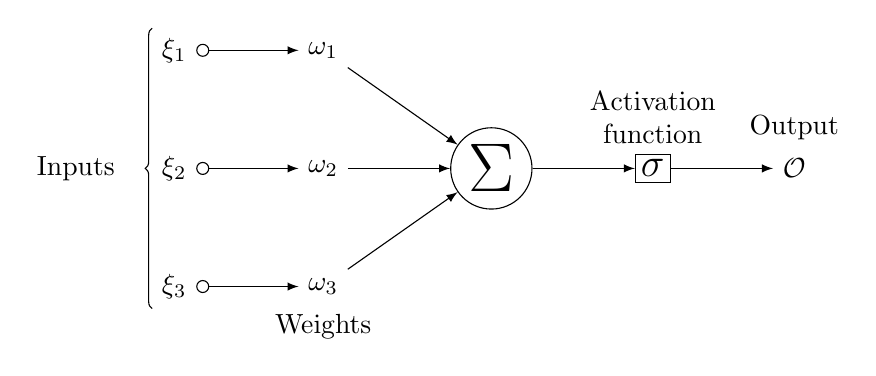
\begin{tikzpicture}[
init/.style={draw, circle, inner sep=2pt, font=\Huge, join = by -latex},
squa/.style={draw, inner sep=2pt, font=\Large, join = by -latex},
start chain=2,node distance=13mm
]
\node[on chain=2] (x2) {$\xi_2$};
\node[on chain=2, join=by o-latex] {$\omega_2$};
\node[on chain=2, init] (sigma) {$\displaystyle\Sigma$};
\node[on chain=2, squa,label=above:{\parbox{2cm}{\centering Activation \\ function}}] {$\sigma$};
\node[on chain=2, label=above:Output,join=by -latex] {$\mathcal{O}$};
\begin{scope}[start chain=1]
  \node[on chain=1] at (0,1.5cm) (x1) {$\xi_1$};
  \node[on chain=1, join=by o-latex] (w1) {$\omega_1$};
\end{scope}
\begin{scope}[start chain=3]
  \node[on chain=3] at (0,-1.5cm) (x3) {$\xi_3$};
  \node[on chain=3, label=below:Weights, join=by o-latex] (w3) {$\omega_3$};
\end{scope}

\draw[-latex] (w1) -- (sigma);
\draw[-latex] (w3) -- (sigma);

\draw[decorate,decoration={brace,mirror}] (x1.north west) -- node[left=10pt] {Inputs} (x3.south west);
\end{tikzpicture}
\end{center}

Understanding now the basic logic behind individual neurons, we turn to the the architecture of a full neural network. In the most basic format, known frequently as a ``feed forward'' network, a neural network contains three types of layers, each of which is a vector of neurons, each taking input from every neuron in the previous layer without interacting with the rest of the layer.
\begin{itemize}
\item{The first layer is the \textbf{input layer}. Input data is fed directly into this layer, and the number of neurons typically is the same as the number of input values.}
\item{Following the input layer comes at least one \textbf{hidden layer} (more than one in deep neural networks). The output values of the neurons in these layers are not necessarily returned to a user, rather, they are passed on to the following layer, which can be the output layer or another hidden layer.}
\item{Neurons in the \textbf{output layer} return the output of the neural network. Note that traditionally, the activation function is implemented here as well, so basic feed forward networks are generally capable only of outputting a value in the range of the chosen activation function.}
\end{itemize}

\begin{center}
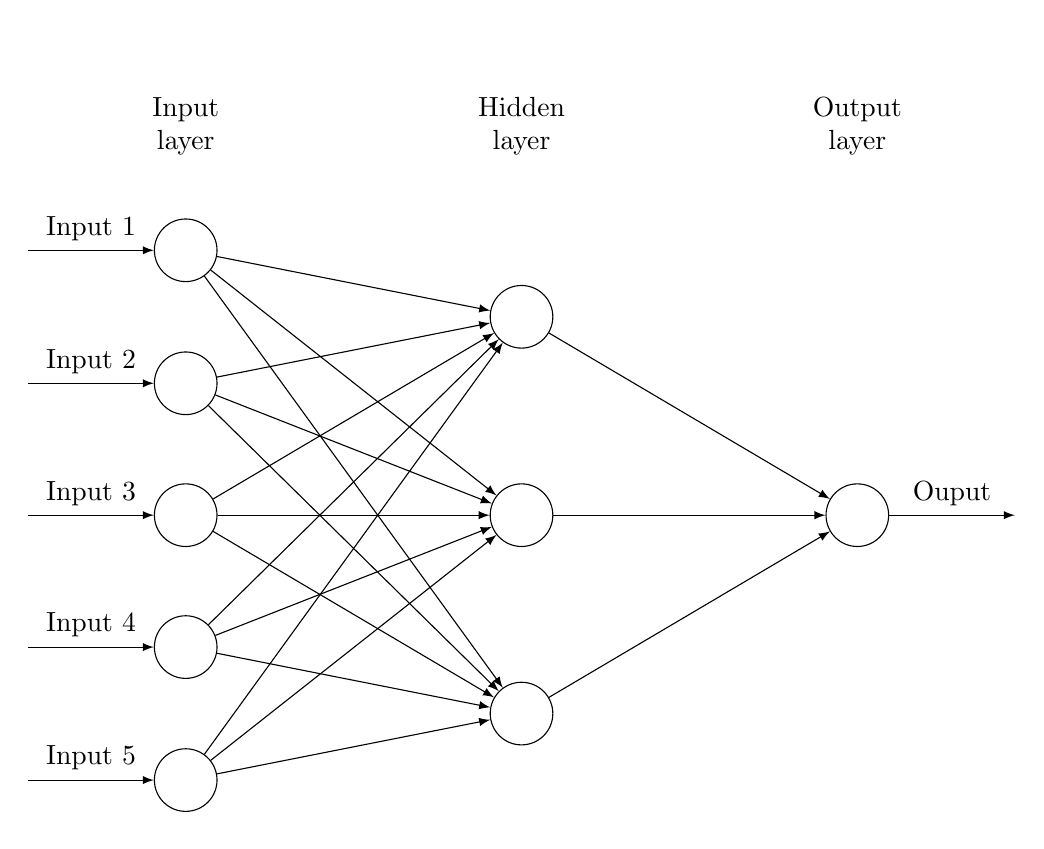
\begin{tikzpicture}[
plain/.style={draw=none, fill=none},
net/.style={matrix of nodes, nodes={draw, circle, inner sep=8pt}, nodes in empty cells, column sep=2cm, row sep=1pt}, >=latex
]
\matrix[net] (mat)
{
|[plain]| \parbox{1.3cm}{\centering Input\\layer} & |[plain]| \parbox{1.3cm}{\centering Hidden\\layer} & |[plain]| \parbox{1.3cm}{\centering Output\\layer} \\
& |[plain]| \\
|[plain]| & \\
& |[plain]| \\
  |[plain]| & |[plain]| \\
& & \\
  |[plain]| & |[plain]| \\
& |[plain]| \\
  |[plain]| & \\
& |[plain]| \\    };
\foreach \ai [count=\mi ]in {2,4,...,10}
  \draw[<-] (mat-\ai-1) -- node[above] {Input \mi} +(-2cm,0);
\foreach \ai in {2,4,...,10}
{\foreach \aii in {3,6,9}
  \draw[->] (mat-\ai-1) -- (mat-\aii-2);
}
\foreach \ai in {3,6,9}
  \draw[->] (mat-\ai-2) -- (mat-6-3);
\draw[->] (mat-6-3) -- node[above] {Ouput} +(2cm,0);
\end{tikzpicture}
\end{center}

\subsection{Backpropogation}
A central component of neural network training is the process of backpropogation. In very general terms, backpropogation is the process of determining the ``error'' of the network, or the difference between outputs the network delivers and desired outputs, during training, and subsequently going backward through the network and adjusting neuron weights and biases accordingly.

To calculate error for an individual output neuron, the process is quite simple: we need only to find the difference between the neuron output $\omega_n$ and the known target value $t_n$.
$$E_n=t_n-\mathcal{O}_n$$
We can then expand this function to find the total error of the network during one epoch (training iteration) as follows. This equation is frequently referred to as the ``cost function.'' [citation needed]
$$C=\frac{1}{2}\sum_n(t_n-\mathcal{O}_n)^2$$
In the context of popular neuroscience (originally in \cite{neuronsfire}), the adage is frequently repeated that ``neurons which fire together, wire together.'' This concept persists in artificial neural networks as well as natural. Through backpropogation, we recursively readjust weights proportionally to their influence on output so as to achieve a more accurate result.

The essence of backpropogation lies in calculating $\frac{\partial{C}}{\partial{\omega}}$ of all weights, or, concretely, the extent to which shifts in each synapse weight affect the final amount of error. Calculating this derivative involves aggressive use of calculus' chain rule.

\section{Appendices}

\label{sec:appendix_a}
\subsection{Appendix A: Scripts for building training data}
Training data for our neural network is retrieved from the Wikimedia Foundation's data dumps in each language. To download and extract the data archives we use a simple bash script \texttt{download.sh}:
\inputminted{bash}{data/download.sh}
We then use a program \texttt{process.py} to extract article text from the complicated dump file and export each language's articles into a single text file which may easily be read by the network during training:
\inputminted{python}{data/process.py}

\bibliography{research}

\end{document}
